\errorcontextlines9999
\documentclass[
	aspectratio=169, 
	10pt 
]{beamer}

\usepackage{fancybeamer} 
\usepackage{fancycolumn}
\usepackage[dvipsnames]{xcolor}
\usepackage{colortbl}
\usepackage{array}
\usepackage{csquotes}
\usepackage{tikz}
\usetikzlibrary{positioning}
\usetikzlibrary{tikzmark}

\newcommand{\harray}[1]{{\color{red}[}#1{\color{red}]}}

\title{Haskell Done Quick (03)} 
\author{Lars Pfrenger} 
\date{07. Februar 2025} 

\lstset{
        classoffset=1, 
        morekeywords={Node, Leaf, Stem, Fruit, Flower, Plant, StackPlant, NODE, LEAF, FLOWER, FRUIT, STEM}, 
        keywordstyle=\color{red}, 
        classoffset=2, 
        morekeywords={plantToStack, stackToPlants}, 
        keywordstyle=\color{Blue}
}

\begin{document}
\maketitle

\section{Stacks}

\subsection{Funktionsweise}
\begin{frame}[t]{\insertsubsection}
    \begin{fancycolumns}[b]
        \alt<1-5>{
		    \begin{info}{Push}Etwas auf den Stack \enquote{legen}\end{info}
        }{
            \begin{ginfo}{Push}Etwas auf den Stack \enquote{legen}\end{ginfo}
        }

        \alt<1,6-9>{
            \begin{info}{Pop}Etwas vom Stack \enquote{nehmen}\end{info}
        }{
            \begin{ginfo}{Pop}Etwas vom Stack \enquote{nehmen}\end{ginfo}
        }
        
        \vspace{1.5cm}
        
        \begin{enumerate}
            \item[$\rightarrow$] Man nehmet/leget nur von \enquote{oben}
            \item[$\rightarrow$] Last In First Out (\textbf{LIFO})
        \end{enumerate}
       
        \nextcolumn
        
        \raggedleft
        \begin{tikzpicture}[squarednode/.style={rectangle, draw=gray!60, fill=gray!5, thick, minimum width=0.8\textwidth, anchor=south}]
            \onslide<2-8>{\node[squarednode](a){1};}
            \onslide<3-7>{\node[squarednode](b)[above=0.2cm of a]{2};}
            \onslide<4-6>{\node[squarednode](c)[above=0.2cm of b]{3};}
            \only<5> {\node[squarednode](d)[above=0.2cm of c]{4};}

            \only<2>{\node at (0,0.61\textheight) {$push(1)$};}
            \only<3>{\node at (0,0.61\textheight) {$push(2)$};}
            \only<4>{\node at (0,0.61\textheight) {$push(3)$};}
            \only<5>{\node at (0,0.61\textheight) {$push(4)$};}
            \only<6>{\node at (0,0.61\textheight) {$pop() \rightarrow 4$};}
            \only<7>{\node at (0,0.61\textheight) {$pop() \rightarrow 3$};}
            \only<8>{\node at (0,0.61\textheight) {$pop() \rightarrow 2$};}
            \only<9>{\node at (0,0.61\textheight) {$pop() \rightarrow 1$};}
        \end{tikzpicture}
	\end{fancycolumns}
\end{frame}


\section{Baum Serialisieren}
\subsection{Baum (Darstellung)}
\begin{frame}[t,fragile]{\insertsubsection}
    \begin{fancycolumns}[c]
        \begin{lstlisting}[gobble=12]
            ;\tikzmarknode{stema}{Stem}; 3.0 (
                Node [ ;\tikzmarknode{nodea}{};
                    Leaf 2, ;\tikzmarknode{leafa}{};
                    ;\tikzmarknode{stemb}{Stem}; 4.0 (;\tikzmarknode{flowera}{Flower}; 0.4), 
                ]
            )
        \end{lstlisting}

    \nextcolumn
    \pause
    \centering
    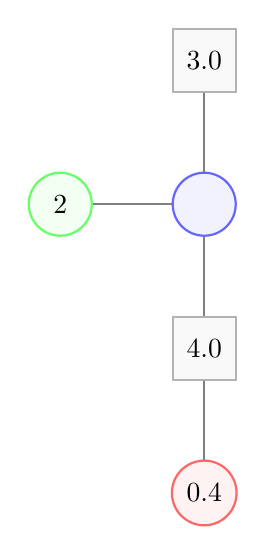
\begin{tikzpicture}[
        stem/.style={rectangle, draw=gray!60, fill=gray!5, thick, minimum size=8mm},
        node/.style={circle, draw=blue!60, fill=blue!5, thick, minimum size=8mm},
        leaf/.style={circle, draw=green!60, fill=green!5, thick, minimum size=8mm},     
        flowr/.style={circle, draw=red!60, fill=red!5, thick, minimum size=8mm},
        remember picture      
    ]
        \node[stem](a){3.0};
            \node[node](b)[below=of a]{};
                \node[stem](c)[below=of b]{4.0};
                   \node[flowr](f)[below=of c]{0.4};
                \node[leaf](d)[left=of b]{2};

        \draw[-, thick, gray] (a.south) -- (b.north);
        \draw[-, thick, gray] (b.south) -- (c.north); 
        \draw[-, thick, gray] (c.south) -- (f.north); 
        \draw[-, thick, gray] (b.west) -- (d.east); 
    \end{tikzpicture}
    \end{fancycolumns}
    
    \begin{tikzpicture}[overlay, remember picture]
        \draw<+(1)->[->, gray] (stema.north) to[out=45,in=180] (a.west);
        \draw<+(1)->[->, blue] (nodea.north) ++(0,0.4ex) to[out=0,in=140] (b.north west);
        \draw<+(1)->[->, green] (leafa.north) ++(0,0.4ex) to[out=0,in=180] (d.west);
        \draw<+(1)->[->, gray] (stemb.south) to[out=270,in=180] (c.west);
        \draw<+(1)->[->, red] (flowera.south) to[out=270,in=180] (f.west);<
    \end{tikzpicture}
\end{frame}

\subsection{Baum zu Stack (Idee)}
\begin{frame}[t, fragile]{\insertsubsection}
    \begin{fancycolumns}[b, widths={40,60}]               
        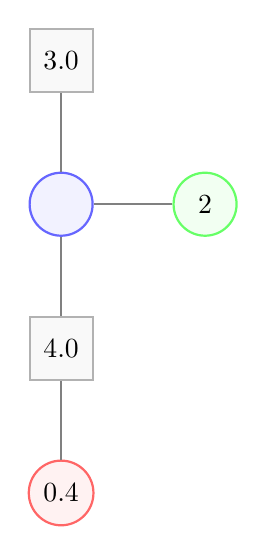
\begin{tikzpicture}[
            stem/.style={rectangle, draw=gray!60, fill=gray!5, thick, minimum size=8mm},
            node/.style={circle, draw=blue!60, fill=blue!5, thick, minimum size=8mm},
            leaf/.style={circle, draw=green!60, fill=green!5, thick, minimum size=8mm},     
            flowr/.style={circle, draw=red!60, fill=red!5, thick, minimum size=8mm},
            remember picture      
        ]
            \node[stem](ga){3.0};
                \node[node](gb)[below=of ga]{};
                    \node[stem](gc)[below=of gb]{4.0};
                       \node[flowr](gf)[below=of gc]{0.4};
                    \node[leaf](gd)[right=of gb]{2};

            \draw[-, thick, gray] (ga.south) -- (gb.north);
            \draw[-, thick, gray] (gb.south) -- (gc.north); 
            \draw[-, thick, gray] (gc.south) -- (gf.north); 
            \draw[-, thick, gray] (gb.east) -- (gd.west); 
        \end{tikzpicture}
        \nextcolumn

        \centering
        \begin{tikzpicture}[squarednode/.style={rectangle, draw=gray!60, fill=gray!5, thick, minimum width=0.8\textwidth, anchor=south}, remember picture]
            \onslide<2->{\node[squarednode](a){STEM 3.0};}
            \onslide<3->{\node[squarednode, draw=blue!60, fill=blue!5](b)[above=0.2cm of a]{NODE 2};}
            \onslide<4->{\node[squarednode, draw=green!60, fill=green!5](c)[above=0.2cm of b]{LEAF 2};}
            \only<5->{\node[squarednode](d)[above=0.2cm of c]{STEM 4.0};}
            \only<6->{\node[squarednode, draw=red!60, fill=red!5](e)[above=0.2cm of d]{FLOWER 0.4};}
            \only<7>{\node[above=1cm of e]{\lstinline{[FLOWER 0.4, STEM 4.0, LEAF 2, NODE 2, STEM 3.0]}};}
        \end{tikzpicture}                
    \end{fancycolumns}

    \begin{tikzpicture}[overlay, remember picture]
        \draw<.(2)>[->, gray] (ga.east) to[out=0,in=180] (a.west);
        \draw<.(3)>[->, blue] (gb.south east) to[out=-45,in=180] (b.west);
        \draw<.(4)>[->, green] (gd.east) to[out=0,in=180] (c.west);
        \draw<.(5)>[->, gray] (gc.east) to[out=0,in=180] (d.west);
        \draw<.(6)>[->, red] (gf.east) to[out=0,in=180] (e.west);
    \end{tikzpicture}
\end{frame}

\subsection{Baum zu Stack (Code)}
\begin{frame}[t, fragile]{\insertsubsection}
    \begin{lstlisting}[gobble=8]
        plantToStack :: Plant leaf flower fruit stem 
            -> [StackPlant leaf flower fruit stem]
        
        plantToStack = foldPlant
            ;\tikzmarknode{fLeaf}{};(\a -> [LEAF a])
            ;\tikzmarknode{fFlower}{};(\a -> [FLOWER a])
            ;\tikzmarknode{fFruit}{};(\a -> [FRUIT a])
            ;\tikzmarknode{fStem}{};(\s p -> p ++ [STEM s])
            ;\tikzmarknode{fNode}{};(\ps -> concat (reverse ps) ++ [NODE (length ps)])
    \end{lstlisting}

    \begin{tikzpicture}[overlay, remember picture]
        \node<2>[above left=-.6ex and 0cm of fLeaf, Gray]{\scriptsize fLeaf};
        \node<3>[above left=-.6ex and 0cm of fFlower, Gray]{\scriptsize fFlower};
        \node<4>[above left=-.6ex and 0cm of fFruit, Gray]{\scriptsize fFruit};
        \node<5>[above left=-.6ex and 0cm of fStem, Gray]{\scriptsize fStem};
        \node<6>[above left=-.6ex and 0cm of fNode, Gray]{\scriptsize fNode};
    \end{tikzpicture}
\end{frame}


\subsection{What the fold doin?}
\begin{frame}[c, fragile]{\insertsubsection \small \color{gray} (post-order-traversal)}
    \begin{tikzpicture}[remember picture, overlay]
        \node[draw, above right=10mm and 5mm] at (current page.south west) (a) {
            \begin{lstlisting}[gobble=16, basicstyle=\tiny]
                plantToStack = foldPlant
                    ;\tikzmarknode{fLeaf}{};(\a -> [LEAF a])
                    ;\tikzmarknode{fFlower}{};(\a -> [FLOWER a])
                    ;\tikzmarknode{fFruit}{};(\a -> [FRUIT a])
                    ;\tikzmarknode{fStem}{};(\s p -> p ++ [STEM s])
                    ;\tikzmarknode{fNode}{};(\ps -> concat (reverse ps) ++ [NODE (length ps)])
            \end{lstlisting}
        };
    \end{tikzpicture}
    \vspace{-1cm}
    \begin{figure}[c]     
        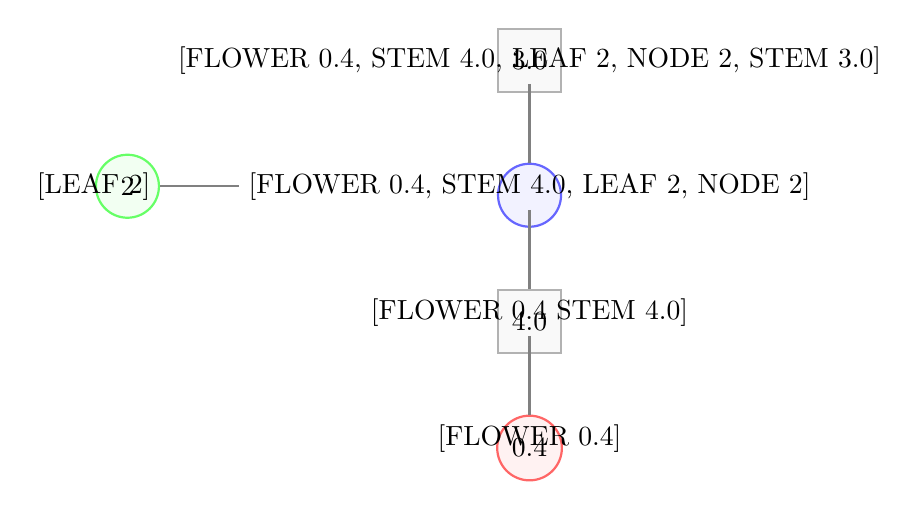
\begin{tikzpicture}[
            stem/.style={rectangle, draw=gray!60, fill=gray!5, thick, minimum size=8mm},
            node/.style={circle, draw=blue!60, fill=blue!5, thick, minimum size=8mm},
            leaf/.style={circle, draw=green!60, fill=green!5, thick, minimum size=8mm},     
            flowr/.style={circle, draw=red!60, fill=red!5, thick, minimum size=8mm},
            remember picture      
        ]
            \node<1-5>[stem](a){3.0};
            \node<6>[](a){\lstinline{[FLOWER 0.4, STEM 4.0, LEAF 2, NODE 2, STEM 3.0]}};


            \node<1-4>[node](b)[below=of a]{};
            \node<5>[](b)[below=of a]{\lstinline{[FLOWER 0.4, STEM 4.0, LEAF 2, NODE 2]}};


            \node<1-3>[stem](c)[below=of b]{4.0};
            \node<4>[](c)[below=of b]{\lstinline{[FLOWER 0.4 STEM 4.0]}};
            
            \node<1-2>[flowr](f)[below=of c]{0.4};
            \node<3>[](f)[below=of c]{\lstinline{[FLOWER 0.4]}};

            \node<1>[leaf](d)[left=of b]{2};
            \node<2-4>[](d)[left=of b]{\lstinline{[LEAF 2]}};


            \draw<1-5>[-, thick, gray] (a.south) -- (b.north);
            \draw<1-4>[-, thick, gray] (b.south) -- (c.north); 
            \draw<1-3>[-, thick, gray] (c.south) -- (f.north); 
            \draw<1-4>[-, thick, gray] (b.west) -- (d.east); 
        \end{tikzpicture}        
    \end{figure}
\end{frame}

\subsection{Stack zu Baum (Idee)}
\begin{frame}[c, fragile]{\insertsubsection}
    \begin{fancycolumns}[c, widths={80,20}]
        \begin{lstlisting}[gobble=12]
            [;\only<1>{FLOWER 0.4, };;\only<-2>{STEM 4.0, };;\only<-3>{LEAF 2, };;\only<-4>{NODE 2, };;\only<-5>{STEM 3.0};]
        \end{lstlisting}
       
        \nextcolumn
        \centering
        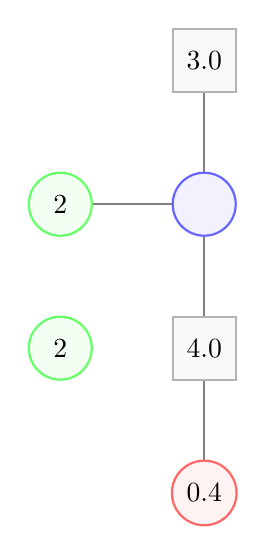
\begin{tikzpicture}[
            stem/.style={rectangle, draw=gray!60, fill=gray!5, thick, minimum size=8mm},
            node/.style={circle, draw=blue!60, fill=blue!5, thick, minimum size=8mm},
            leaf/.style={circle, draw=green!60, fill=green!5, thick, minimum size=8mm},     
            flowr/.style={circle, draw=red!60, fill=red!5, thick, minimum size=8mm},
            remember picture      
        ]
            \node<2->[flowr](f){0.4};
            \node<3->[stem](c)[above=of f]{4.0};
            \node<4>[leaf](d)[left=of c]{2};
            \node<5->[node](b)[above=of c]{};
            \node<5->[leaf](d)[left=of b]{2};
            \node<6->[stem](a)[above=of b]{3.0};
    

            \draw<3->[-, thick, gray] (c.south) -- (f.north); 
            \draw<5->[-, thick, gray] (b.south) -- (c.north); 
            \draw<5->[-, thick, gray] (b.west) -- (d.east); 
            \draw<6->[-, thick, gray] (a.south) -- (b.north);
        \end{tikzpicture}
    \end{fancycolumns}
\end{frame}

\subsection{Stack zu Baum (Code)}
\begin{frame}[c, fragile]{\insertsubsection}
    \begin{lstlisting}[gobble=8]
        stackToPlants :: [StackPlant leaf flower fruit stem] 
            -> [Plant leaf flower fruit stem]
            
        stackToPlants = foldl
            (\ps c -> case c of
                LEAF l -> Leaf l : ps
                FLOWER f -> Flower f : ps
                FRUIT f -> Fruit f : ps
                STEM s -> Stem s (head ps) : tail ps
                NODE n -> Node (take n ps) : drop n ps)
            []
    \end{lstlisting}
\end{frame}

\subsection{What the fold doin (the sequel)}
\begin{frame}[c, fragile]{\insertsubsection}
    \begin{fancycolumns}
        \centering
        \begin{lstlisting}[gobble=8]    
            [FLOWER 0.4, STEM 4.0,
             LEAF 2, NODE 2, STEM 3.0]   
        \end{lstlisting}
        \nextcolumn    
        \centering
        \begin{lstlisting}[gobble=8]     
            []
        \end{lstlisting}
    \end{fancycolumns}
\end{frame}

\begin{frame}[c, fragile]{\insertsubsection}
    \begin{fancycolumns}
        \centering
        \begin{lstlisting}[gobble=8]    
            [STEM 4.0,
             LEAF 2, NODE 2, STEM 3.0]   
        \end{lstlisting}
        \nextcolumn    
        \centering
        \begin{lstlisting}[gobble=8]     
            [Flower 0.4]
        \end{lstlisting}
    \end{fancycolumns}
\end{frame}

\begin{frame}[c, fragile]{\insertsubsection}
    \begin{fancycolumns}
        \centering
        \begin{lstlisting}[gobble=8]    
            [LEAF 2, NODE 2, STEM 3.0]   
        \end{lstlisting}
        \nextcolumn    
        \centering
        \begin{lstlisting}[gobble=8]     
            [(Stem 4.0 (Flower 0.4))]
        \end{lstlisting}
    \end{fancycolumns}
\end{frame}

\begin{frame}[c, fragile]{\insertsubsection}
    \begin{fancycolumns}[widths={40,60}]
        \centering
        \begin{lstlisting}[gobble=8]    
            [NODE 2, STEM 3.0]   
        \end{lstlisting}
        \nextcolumn    
        \centering
        \begin{lstlisting}[gobble=8]     
            [Leaf 2, (Stem 4.0 (Flower 0.4))]
        \end{lstlisting}
    \end{fancycolumns}
\end{frame}

\begin{frame}[c, fragile]{\insertsubsection}
    \begin{fancycolumns}[widths={30,70}]
        \centering
        \begin{lstlisting}[gobble=8]    
            [STEM 3.0]   
        \end{lstlisting}
        \nextcolumn    
        \centering
        \begin{lstlisting}[gobble=8]     
            [(Node [Leaf 2, (Stem 4.0 (Flower 0.4))])]
        \end{lstlisting}
    \end{fancycolumns}
\end{frame}


\begin{frame}[c, fragile]{\insertsubsection}
    \begin{fancycolumns}[widths={10,90}]
        \centering
        \begin{lstlisting}[gobble=8]    
            []   
        \end{lstlisting}
        \nextcolumn    
        \centering
        \begin{lstlisting}[gobble=8]     
            [(Stem 3.0 (Node [Leaf 2, (Stem 4.0 (Flower 0.4))]))]
        \end{lstlisting}
    \end{fancycolumns}
\end{frame}



\end{document}
